\documentclass[a4paper,11pt]{article}
\usepackage[margin=2cm]{geometry}
\usepackage{anysize}
\usepackage[pdftex]{graphicx}
\usepackage{url}
\usepackage{listings}
\usepackage{textcomp}
\usepackage{wrapfig}
\usepackage{color}
\usepackage{fancyhdr}
\usepackage[nodayofweek]{datetime}
\usepackage[small,compact]{titlesec}
\usepackage[pdfborder=0]{hyperref}
\longdate

\setlength{\parskip}{10pt} 
\setlength\parindent{0pt}
\pagestyle{fancyplain}
\fancyhf{}
\lhead{\fancyplain{}{M.Sc.\ Group Project Report}}
\rhead{\fancyplain{}{\today}}
\cfoot{\fancyplain{}{\thepage}}


\title{Twitter for traffic\\\Large{--- Report One ---}}
\author{Porfyrios Vasileiou, Marianna Polatoglou, Afxentios Hadjiminas,\\
        Panagiotis Tsirigotis, Hanguang Zhou, John Flanagan.\\
       \{pv311, mp1911, ah2411, pt1111, hz511, jf311.\}@doc.ic.ac.uk\\ \\
       \small{Supervisor: Dr.\ Emil Lupu, Dr.\ Alessandra Russo, Luke Dickens}\\
       \small{Course: CO533, Imperial College London}
}



%Report details http://www.doc.ic.ac.uk/~cristic/teaching/MScGroupProj/

\begin{document}
\maketitle

\section{Introduction}
	City planners have been struggling to acquire real-time data on traffic
conditions. This data is especially important with incidents which may
translate into traffic disruptions on an already over capacity road network.
Cities have experimented with traffic cameras, dynamic traffic light control
and more traditionally traffic based radio stations.

Internet connected mobile phones and micro-blogging platforms like Twitter have
been providing researchers with a vast and interesting source of real-world
data. This data has been used to analyse trends, identify concepts and to
augment traditional curated data providing a level of social knowledge to the
topic.

Twitter for traffic aims to take these concepts to provide the mobile user with
an application for assessing traffic disruptions as they evolve for London
city. To provide this insight, the application will present the user with
curated traffic disruptions augmented with social knowledge of the event
harvested from a social network.  In addition to this curated list of traffic
disruptions, the concept of identifying emerging disruptions from this social
data will be explored, with the aim of identifying clusters of disruption
reports to discover new disruption events.

To promote the of reporting the traffic conditions on a social network, it will
also be necessary to provide a fast, simple and descriptive mechanism for the
user to manually contribute their observations.

There are a number of interesting challenges the comprise this task. Initially
we must identify tweets from Twitter that discuss road traffic. For these
traffic tweets to be of value we must be able to infer some geographic location
for each tweet, a small percentage of tweets actually contain a geographic
    location so other methods must be explored. To identify events from tweets
    alone, we must investigate geographic clusters of tweets which discuss
    traffic. There are a number of problems in detecting valid traffic
    effecting events, these include sufficient data, timeliness of the tweets
    and  ‘normal’ levels of background chatter.

    From the onset there are many unknowns relating to the data analysis,
    including the quantity of traffic related messages and quality of the
    content. Aspects of this project include data mining, social network
    analysis, mobile application development, document classification and
    geographical information systems.


\section{Requirements}
	Twitter for traffic aims to provide the mobile user with an application for assessing traffic disruptions as they evolve. To provide this insight, the application will present the user with curated traffic disruptions augmented with social knowledge of the event harvested from a social network.

The project will consist of two separate development efforts, consisting of a hosted application to source and correlate data and a mobile application to display events and report disruptions. In order to describe the system, the requirements were identified with goal-oriented capture\cite{Requirements}.

\begin{figure}[here]
\begin{center}
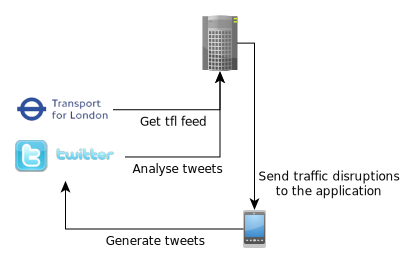
\includegraphics[width=0.7\textwidth]{images/draft_architecture.jpg}
\end{center}
\caption{Application Architecture}
\end{figure}

The hosted application will retrieve traffic events from a Transport for London (TfL) data feed and correlate each event with relevant tweets harvested from Twitter. The server based application gathers data from TfL and Twitter periodically. TfL provides a curated feed of ongoing traffic disruptions in a structured format. Twitter provides us with a torrent of unsorted tweets, from which relevant tweets must be extracted. In addition traffic disruptions reported from the mobile application can be identified through the use of a hash tag, enabling these messages to be processed separately. The server gathers the TfL data and then tries to match tweets about these traffic disruptions. To discover tweets that discuss traffic concepts, document classification techniques must be utilised. Two points we can improve on the server is the classification algorithm, and adding the functionality to generate traffic disruptions that are reported only from Twitter, and not yet on TfL.

The mobile application must provide the commuter with a mechanism for discovering disruptions that may affect their route. This is to be provided through the use of a map based interface. In addition the mobile application must offer the user the ability to comment or describe an on going traffic disruption. The user interface for reporting disruptions must offer a quick and intuitive mechanism for describing a particular event, while also satisfying users that require more control over the messages published on their account.

Below there are tables for every feature and its priority, feasibility and expected completion date. The smaller number in priority means more important to finish fast (1-10) and in feasibility the smaller number means more achievable (1-10).

\begin{center}
\begin{tabular}{ | p{6cm} | c | c | c | }
\hline
\multicolumn{4}{|c|}{\textbf{Server Hosted Application}} \\ \hline
\textbf{Feature} & \textbf{Priority} & \textbf{Feasibility} & \textbf{Expected completion} \\ \hline
\textbf{Store current disruptions from TfL} \newline
Create a geographic database of live events from TfL. Evolve these database events with data from the feed, in order to have a current representation of the event. & 1 & 3 & \\ \hline
\textbf{Classify tweets from Twitter with a simple classifier}
Identify traffic related tweets with a simple classifier and store those tweets, using their geographic representation as a key. & 2 & 3 & \\ \hline
\textbf{Store tweets} \newline
Store relevant tweets using their geographical representation as a key. & 2 & 2 & \\ \hline
\textbf{Implement better classification algorithm} \newline
Use an algorithm that will give better results, while the trade-off with the classification time will not be that high. & 4 & 6 & \\ \hline
\textbf{Generate traffic disruptions from Twitter} \newline
Analyse incoming traffic tweets and determine new non-TfL disruptions from those. & ? & ? & \\ \hline
\textbf{Process mobile client reports} \newline
Take twitter messages reported from the mobile client and process these in a separate pipeline. & ? & ? & \\ \hline
\end{tabular}
\end{center}

\begin{center}
\begin{tabular}{ | p{6cm} | c | c | c | }
\hline
\multicolumn{4}{|c|}{\textbf{Mobile Application}} \\ \hline
\textbf{Feature} & \textbf{Priority} & \textbf{Feasibility} & \textbf{Expected completion} \\ \hline
\textbf{Report events}
Report traffic disruption through the mobile application on Twitter, using a hash tag. & 1 & 2 & \\ \hline
\textbf{Show local disruption map}
Show positions of known disruptions a map. Enabling the user to click on a particular event for further information. & 1 & 2 & \\ \hline
\textbf{Stored Routes}
Find and show disruptions for user defined stored routes. & 3 & 5 & \\ \hline
\end{tabular}
\end{center}

\section{Development Methodology}
	To begin identifying an appropriate development methodology, it is necessary to understand the project requirements. The project requirements and features are determined over a number of meetings with the primary stakeholders. 

At this point, the development methodology can be determined. Since we are looking for iterative and incremental development, Agile Software Development Methodology will be followed. This also enables time-boxed iterative approach. Agile methods are focused on different aspects of the software development life cycle. Two of the most well known agile methodologies are Scrum and XP.

Scrum is an agile project management technique that focuses more on the management of software development projects. The product is completed in a series of one to four week iterations, or sprints. Before each sprint, a planning meeting is held to define which features will be implemented during that sprint. Similarly, XP (Extreme Programming) is an agile methodology which is designed for small, co-located teams aiming to get quality and productivity as high as possible. It does this through the use of rich, short, informal communication paths with emphasis on skill, discipline, and understanding at the personal level, minimizing all intermediate work products.

As this is a college project and tight time constraints apply, it is quite
difficult to follow a particular methodology. Scrum focuses on the management
side of the project whereas XP focuses more on the actual programming
practices. It is more preferable if various elements from both methodologies
can be used, since they address different areas and complement each other.

Therefore, it was decided to focus on managing the software project using the scrum
approach and adopt characteristics that suit the project. Weekly meetings are planned to organise the division
of work and for the team to get up to speed with all the tasks in progress and recently
completed. An agenda for each meeting is stored in an online document, that
each team member may add to. 

To encourage a more agile development the online collaboration tool
Trello is used. This tool gives access to a visual board that displays the
on going tasks. These tasks are represented as cards with labels and priorities. 
Trello is very similar in concept to the scrum board, as shown in fig 2.

\begin{figure}[here]
\begin{minipage}{\textwidth}  
\begin{center}
\includegraphics[width=0.95\textwidth]{images/scrumboard.jpg}
\end{center}
\vspace{-20pt}
\caption[Caption for LOF]{Scrum Board and Trello\footnotemark}
\end{minipage} 
\end{figure}
\footnotetext{Left: Drew Stephens \url{flickr.com/photos/dinomite/3695570625}, Right: \copyright \url{Trello.com}}

It was agreed that adopting techniques from XP would help to
improve the development process. Pair programming is one of those techniques the team would strive to adopt.
Two programmers work alongside on the same code and together they develop a single feature. Constant refactoring is another key practice to be adopted. Any
time the two find a section of code that appears hard to understand or overly
complex, they are to revise it, constantly simplifying and improving it. Furthermore, a test driven approach will be taken during this development.
However because of the nature of the project being partly research based and
the results being quite subjective, it is difficult to test effectively. Hence,
the development of the mobile application will be test-driven whereas for the
server development it will not be possible to follow test driven approach so strictly\cite{Cockburn}. These techniques improve the code quality and team focus.

For the division of work amongst the team, more flexibility will be achieved by maximising the use of the members previous experience. A division has been decided where two members of the team will focus on the mobile application, three on the server side and the final person will move between these tasks as necessary. A team leader is also designated with the aim of coordinating the two development efforts.  

To achieve parallel development, the server API will be agreed and mocked-up returning a static data set. That way, those developing the mobile application can work independently from those working on the server.

The mobile application is the only user facing aspect of the project. The user interface will be agreed using a series of LoFi (pen and paper) concepts, to prove that they provide the required features in a user friendly manner.



\section{Revision Control}
	Management of source-code, documentation and binary files can be tedious for an individual, but when you consider a team working on a set of files, tracking changes and version becomes close to impossible.

While many different approaches are used to track files, most revision control systems offer
similar basic functionality. This main functionality could be described under
the title of ‘collaboration’, enabling multiple individuals to work on as set of
files while ensuring changes don’t get lost and enabling tracking of versions.
Modern systems offer powerful features such as verifiable histories, ability to integrate with deployment, test and code review systems and the ability to add rules to enforce corporate policy and process.

The chosen revision control system needs to be free and preferably open-source,
work well in a disconnected environment, have good documentation and also
beneficial if this tool is in common use. Git\cite{website:git_scm}, the
open-source distributed revision control system used by many major projects
including the Linux Kernel, Google’s Androida and Eclipse seemed to meet the
teams requirements. Additionally, members of the team have previous experience using the tool, which will lessen the initial learning curve.

The distributed nature of Git means a centralised ‘server’ is not necessary,
but for convenience Github\cite{website:github} an online hosting service for
git is to be utilised. In addition to hosting the repository, Github offers a
simple user interface for browsing the history, project bug-tracking, wiki, and
is free for public projects with less the 300mb of history. However, using
Github means we lose the ability to interface with git hooks on the server. 

From the beginning of the project it was agreed that all data will exist
outside of the repository. This was enforced by policy and by using a ‘.gitignore’ file in the root of the repository to list file types to be not tracked.  

To extract as much value as possible from revision control it is important to
make commit messages as concise and descriptive as possible. The book Pro
Git\cite{website:pro_git_ch2} describes a good commit as having the folloing
structure; break the message into a brief 50 character summary insert a new line and a more detailed
description. Enforcing good commit messages will help any team member to
quickly look at the commit log and understand the current state of development.
It is also important not get too wrapped up in these aspects, and keep the development somewhat agile.

The team’s repository is available at: \url{https://github.com/johnflan/Twitter-4-Traffic}
\pagebreak 


\section{References}
	\vspace{-20pt}
	\def\refname{}
	\bibliography{references}
	\bibliographystyle{plain}

\end{document}
